% Author: Izaak Neutelings (August 2023)
% Description: Vertex reconstruction of two photon decay
% https://indico.cern.ch/event/1296197/#4-exo-23-012-search-for-displa
\documentclass[border=3pt,tikz]{standalone}
\usepackage{amsmath}
\usepackage[outline]{contour} % glow around text
\usetikzlibrary{calc}
\usetikzlibrary{decorations.pathmorphing} % for snake, coil, zigzag
\usetikzlibrary{angles,quotes} % for pic (angle labels)
\tikzset{>=latex} % set default arrow head as latex
\contourlength{1.1pt}

% COLORS
\colorlet{myblue}{blue!80!black}
\colorlet{mygreen}{green!80!black}
\colorlet{calocol}{blue!60!green!90!black!70}
\colorlet{photoncol}{yellow!60!orange!95!black}

% STYLES
\tikzstyle{circle}=[mygreen,dashed]
\tikzstyle{calo}=[draw=calocol!40!black,fill=calocol,
                  line width=0.6,rounded corners=0.4pt] % calorimeter deposit
\tikzstyle{MET}=[->,red,line width=1.2,dashed]
\tikzstyle{photon}=[thick,line cap=round,photoncol,decorate,decoration={
  snake,amplitude=.4mm,segment length=2.5mm,post length=1mm}]

% MACROS
\newcommand*{\myvec}[1]{\vec{\mkern0mu#1}} % correct misalignment in \vec
\newcommand{\ptmiss}{\myvec{p}_\mathrm{T}^\mathrm{\,miss}}
\def\compute{ % compute all vertex parameters
  \pgfmathsetmacro\l{sqrt(\R^2-(\L)^2*sin(\atheta/2)^2)-\L*cos(\atheta/2)} % length photon (diphoton vertex to ECAL deposit)
  \pgfmathsetmacro\p{\l*cos(\atheta/2)} % projection photon on bisector
  \pgfmathsetmacro\r{\l/(2*cos(\atheta/2))} % radius of diphoton circle
  \pgfmathsetmacro\aphip{acos((\L+\p)/\R)} % azimuthal angle between photon and bisector from vertex
  \message{^^JDiphoton opening angle theta = \atheta}
  \message{^^JECAL inner radius R = \R}
  \message{^^JParticle path length L = \L}
  \message{^^JPhoton path length l = \l}
  \message{^^JProj. photon length p = \p}
  \message{^^JPhi photon-bisector aphi = \aphip}
}

\begin{document}


% VERTEX RECONSTRUCTION
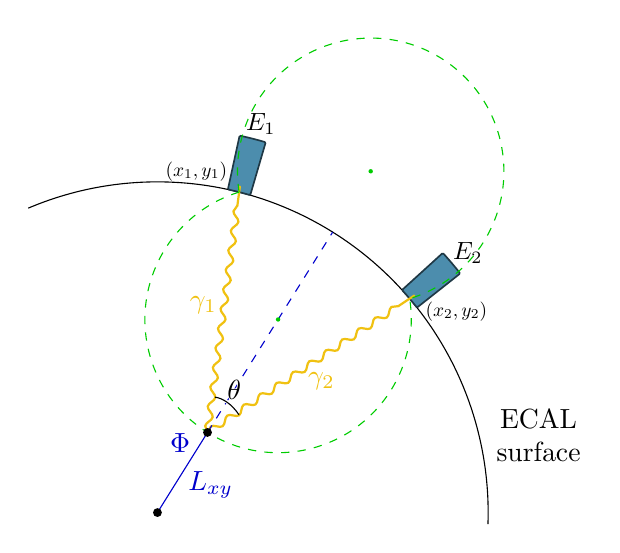
\begin{tikzpicture}[rotate=0]
  \def\R{4.2}     % tracker outer radius
  \def\L{1.2}     % distance between PV and diphoton vertex
  \def\aphi{58}   % direction diphoton system (pho)
  \def\atheta{49} % opening angle between photons (theta)
  \def\aECAL{4}   % angular granularity of calo deposits, CMS: 0.0175*180/pi = 1
  \compute        % compute all vertex parameters
  
  % COORDINATES
  \coordinate (O) at (0,0);      % detector center
  \coordinate (V) at (\aphi:\L); % diphoton vertex
  \coordinate (P) at (\aphi:\R); % projection of diphoton vertex
  \coordinate (C1) at (\aphi:\L+\r); % circle center inside
  \coordinate (C2) at (\aphi:{\L+2*\p-\r}); % circle center outside
  \coordinate (P1) at ($(V)+(\aphi+\atheta/2:\l)$); % photon 1 at ECAL
  \coordinate (P2) at ($(V)+(\aphi-\atheta/2:\l)$); % photon 2 at ECAL
  
  % CALORIMETER INNER SURFACE
  \draw (\aphi-60:\R) arc (\aphi-60:\aphi+55:\R);
  %\draw circle (\R);
  \node[anchor=-150,inner sep=4pt,align=center] at (\aphi-50:\R)
    {ECAL\\surface};
  
  % CALORIMETER DEPOSITS
  \def\drawdepo#1#2{
    \draw[calo]
      (#1+\aECAL/2:\R+#2) arc(#1+\aECAL/2:#1-\aECAL/2:\R+#2) node (Ce) {}
      -- (#1-\aECAL/2:\R) arc(#1-\aECAL/2:#1+\aECAL/2:\R) -- cycle;
  }
  \drawdepo{\aphi+\aphip}{0.7}
  \node[anchor=\aphi+\aphip+210,inner sep=3pt,scale=0.9] at (Ce)
    {$E_1$};
  \node[anchor=\aphi-84,inner sep=6pt,scale=0.7] at (P1)
    {$(x_1,y_1)$};
  \drawdepo{\aphi-\aphip}{0.7}
  \node[anchor=\aphi-\aphip+210,inner sep=4pt,scale=0.9] at (Ce)
    {$E_2$};
  \node[anchor=\aphi+107,inner sep=8pt,scale=0.7] at (P2)
    {$(x_2,y_2)$};
  
  % LINES
  \draw[photon,shorten >=-2pt] (V) -- (P1) % photon 1
    node[midway,anchor=-20,inner sep=2pt] {$\gamma_1$};
  \draw[photon,shorten >=-2pt] (V) -- (P2) % photon 2
    node[midway,anchor=130,inner sep=2pt] {$\gamma_2$};
  \draw[myblue] (O) -- (V) % path of instable particle Phi -> aa
    node[pos=0.75,anchor=\aphi-90,inner sep=1.6pt] {$\Phi$}
    node[pos=0.55,anchor=\aphi+90,inner sep=1.0pt] {$L_{xy}$}; %\mathrm{3D}
  \draw[myblue,dashed] (V) -- (P); % bisector
  %\draw[red] (O) -- (\aphi+\aphip:\R);
  %\draw[red] (O) -- (\aphi-\aphip:\R);
  %\draw[red] (P1) -- (P2);
  %\fill[red] (V)++(\aphi:\p) circle(1pt);
  %\draw[orange] (O) -- (P1);
  %\draw[orange] (O) -- (P2);
  
  % OPENING ANGLE
  \draw pic[draw=white,very thick,shorten >=1.8pt,shorten <=0.5pt,
    angle radius=13,angle eccentricity=1.4]
    {angle = P2--V--P1}; % while contour line
  \draw pic["\contour{white}{$\theta$}",draw=black,
    shorten >=1.0pt,shorten <=-1.0pt,angle radius=13,angle eccentricity=1.4]
    {angle = P2--V--P1};
  
  % CIRCLES (for vertex reconstruction)
  \fill[mygreen] (C1) circle(0.8pt);
  \fill[mygreen] (C2) circle(0.8pt);
  %\draw[red]
  %  (C1) circle(\r)
  %  (C2) circle(\r);
  %\draw[green]
  %  (C1) --++ (\aphi+\atheta:\r)
  %  (C2) --++ (\aphi-\atheta+180:\r)
  %  (C1) --++ (\aphi+180:\r)
  %  (C2) --++ (\aphi:\r);
  \draw[circle,dashed] % inside circle
    (P1) arc({\aphi+\atheta}:{\aphi+360-\atheta}:{\r});
  \draw[circle,dashed] % outside circle
    (P1) arc({\aphi-\atheta+180}:{\aphi-180+\atheta}:{\r});
  
  % VERTICES
  \fill (O) circle(1.6pt);
  \fill (V) circle(1.6pt);
  
\end{tikzpicture}


% VERTEX RECONSTRUCTION (background)
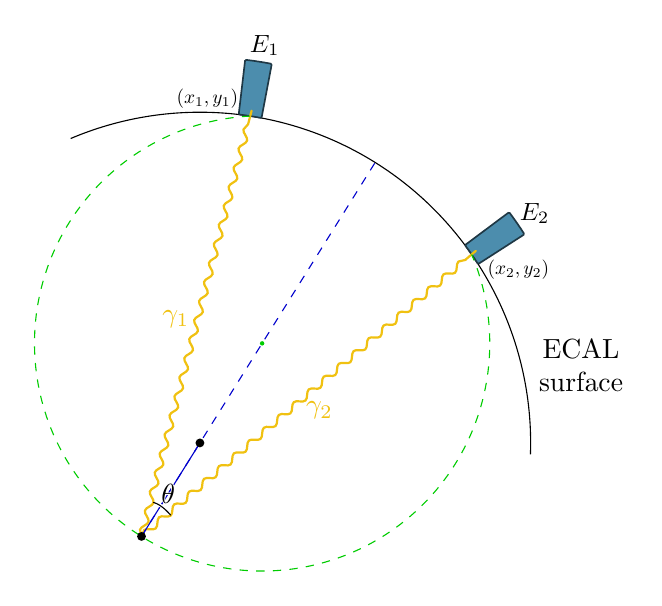
\begin{tikzpicture}[rotate=0]
  \def\R{4.2}     % tracker outer radius
  \def\L{-1.4}    % distance between PV and diphoton vertex
  \def\aphi{58}   % direction diphoton system (pho)
  \def\atheta{35} % opening angle between photons (theta)
  \def\aECAL{4}   % angular granularity of calo deposits, CMS: 0.0175*180/pi = 1
  \compute        % compute all vertex parameters
  
  % COORDINATES
  \coordinate (O) at (0,0);      % detector center
  \coordinate (V) at (\aphi:\L); % diphoton vertex
  \coordinate (P) at (\aphi:\R); % projection of diphoton vertex
  \coordinate (C1) at (\aphi:\L+\r); % circle center inside
  \coordinate (P1) at ($(V)+(\aphi+\atheta/2:\l)$); % photon 1 at ECAL
  \coordinate (P2) at ($(V)+(\aphi-\atheta/2:\l)$); % photon 2 at ECAL
  
  % CALORIMETER INNER SURFACE
  \draw (\aphi-60:\R) arc (\aphi-60:\aphi+55:\R);
  \node[anchor=-150,inner sep=4pt,align=center] at (\aphi-50:\R)
    {ECAL\\surface};
  
  % CALORIMETER DEPOSITS
  \def\drawdepo#1#2{
    \draw[calo]
      (#1+\aECAL/2:\R+#2) arc(#1+\aECAL/2:#1-\aECAL/2:\R+#2) node (Ce) {}
      -- (#1-\aECAL/2:\R) arc(#1-\aECAL/2:#1+\aECAL/2:\R) -- cycle;
  }
  \drawdepo{\aphi+\aphip}{0.7}
  \node[anchor=\aphi+\aphip+210,inner sep=3pt,scale=0.9] at (Ce)
    {$E_1$};
  \node[anchor=\aphi-80,inner sep=6pt,scale=0.7] at (P1)
    {$(x_1,y_1)$};
  \drawdepo{\aphi-\aphip}{0.7}
  \node[anchor=\aphi-\aphip+210,inner sep=4pt,scale=0.9] at (Ce)
    {$E_2$};
  \node[anchor=\aphi+104,inner sep=8pt,scale=0.7] at (P2)
    {$(x_2,y_2)$};
  
  % LINES
  \draw[photon,shorten >=-2pt] (V) -- (P1) % photon 1
    node[midway,anchor=-20,inner sep=2pt] {$\gamma_1$};
  \draw[photon,shorten >=-2pt] (V) -- (P2) % photon 2
    node[midway,anchor=130,inner sep=2pt] {$\gamma_2$};
  \draw[myblue] (O) -- (V); % path of instable particle
  \draw[myblue,dashed] (V) -- (P); % bisector
  
  % OPENING ANGLE
  \draw pic[draw=white,very thick,shorten >=1.8pt,shorten <=0.5pt,
    angle radius=13,angle eccentricity=1.4]
    {angle = P2--V--P1}; % while contour line
  \draw pic["\contour{white}{$\theta$}",draw=black,
    shorten >=1.0pt,shorten <=-1.0pt,angle radius=13,angle eccentricity=1.4]
    {angle = P2--V--P1};
  
  % CIRCLES (for vertex reconstruction)
  \fill[mygreen] (C1) circle(0.8pt);
  \draw[circle,dashed] % inside circle
    (P1) arc({\aphi+\atheta}:{\aphi+360-\atheta}:{\r});
  
  % VERTICES
  \fill (O) circle(1.6pt);
  \fill (V) circle(1.6pt);
  
\end{tikzpicture}


\end{document}